\chapter{Results}\label{ch:Results}
This chapter presents the simulation results and a comparison between all proposed methods in different scenarios variating from low to high weed density infestation. The goal of this chapter is to come up with the best solution for the task allocation problem and measure the performance improvement over the baseline method.

Paltech currently offers its weeding solutions in fields ranging from $0.5$ to $20$ hectares, with an average weed density of $0.4$ to $1.0$ weeds/m$^2$. \autoref{fig:field-weed-density} shows an example of weed density in a 1-hectare field, while \autoref{fig:field-path-planning} illustrates the coverage path planning pattern that the robot follows in the same field. The simulations in this thesis are limited to the linear movements shown in \ref{fig:field-path-planning}, due to the motion constraints described at the beginning of chapter \ref{ch:TA}. As a result, the simulation environments are designed accordingly.

\begin{figure}[htb]
    \myfloatalign
    \subfloat[Weed density]
    {\label{fig:field-weed-density}
        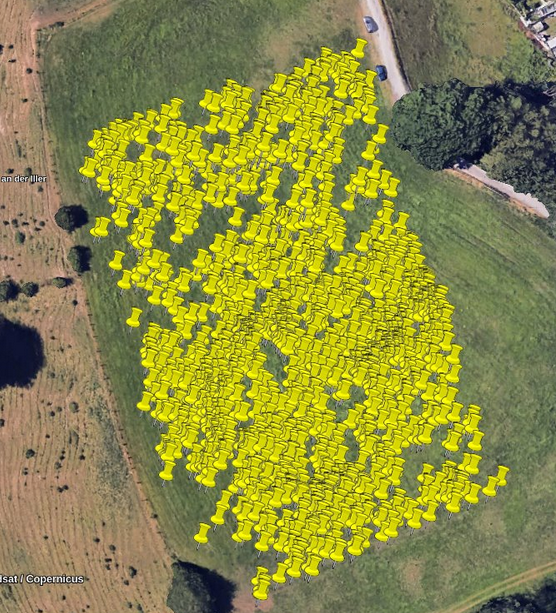
\includegraphics[width=.41\linewidth]{gfx/ch04/field_weed_density.png}} \quad
    \subfloat[Coverage path planning pattern]
    {\label{fig:field-path-planning}%
        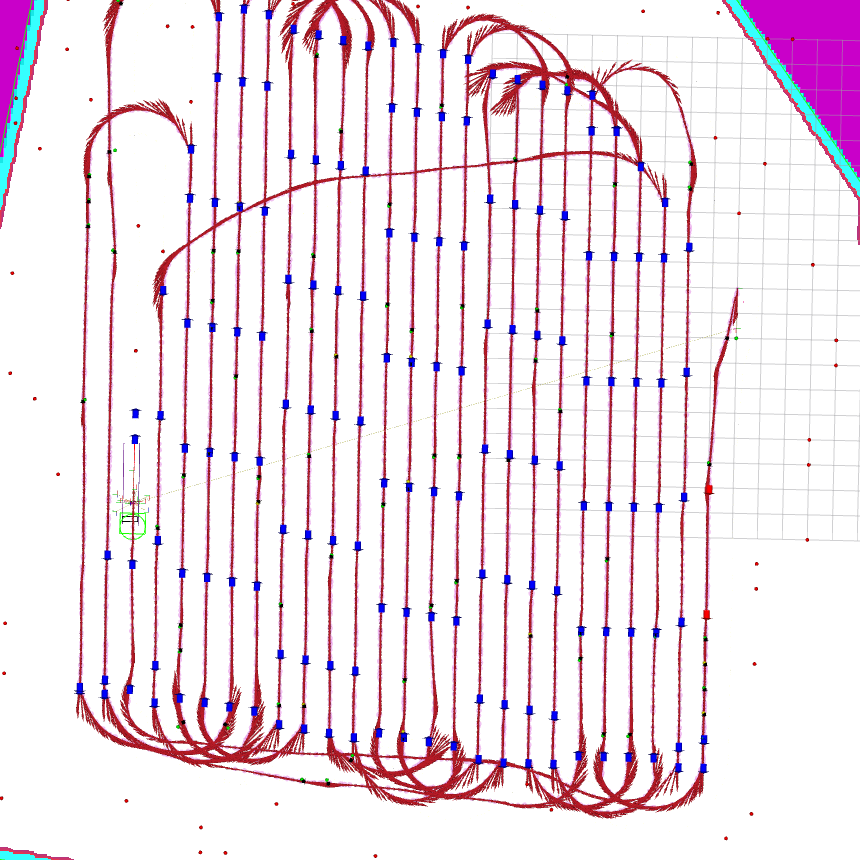
\includegraphics[width=.45\linewidth]{gfx/ch04/field_path_planning.png}} \\
    \caption{Weed distribution and coverage path in an agricultural field}\label{fig:usual-field-example}
\end{figure}

\section{Simulation Setup}
Simulated worlds were customized using YAML files, as mentioned in \autoref{sec:simulation}, allowing for repeatability and ease of configuration. The first scenario consisted of a rectangular area with dimensions $2,\text{m} \times 50,\text{m}$, totaling $100,\text{m}^2$, and an average weed density of $0.88$ weeds/m$^2$. The local distribution per quadrant ($2,\text{m} \times 2,\text{m}$) varied in both type (\textit{uniform or clustered}) and density. The first comparison was made between the heuristic baseline method using one and two tools. This comparison was made only to determine the natural improvement of mission time reduction when adding an additional tool even with a non-optimized algorithm. \autoref{} displays the 

\begin{figure}[htb]
    \myfloatalign
    \subfloat[Mission Metrics]
    {\label{fig:heuristics-1-mission}
        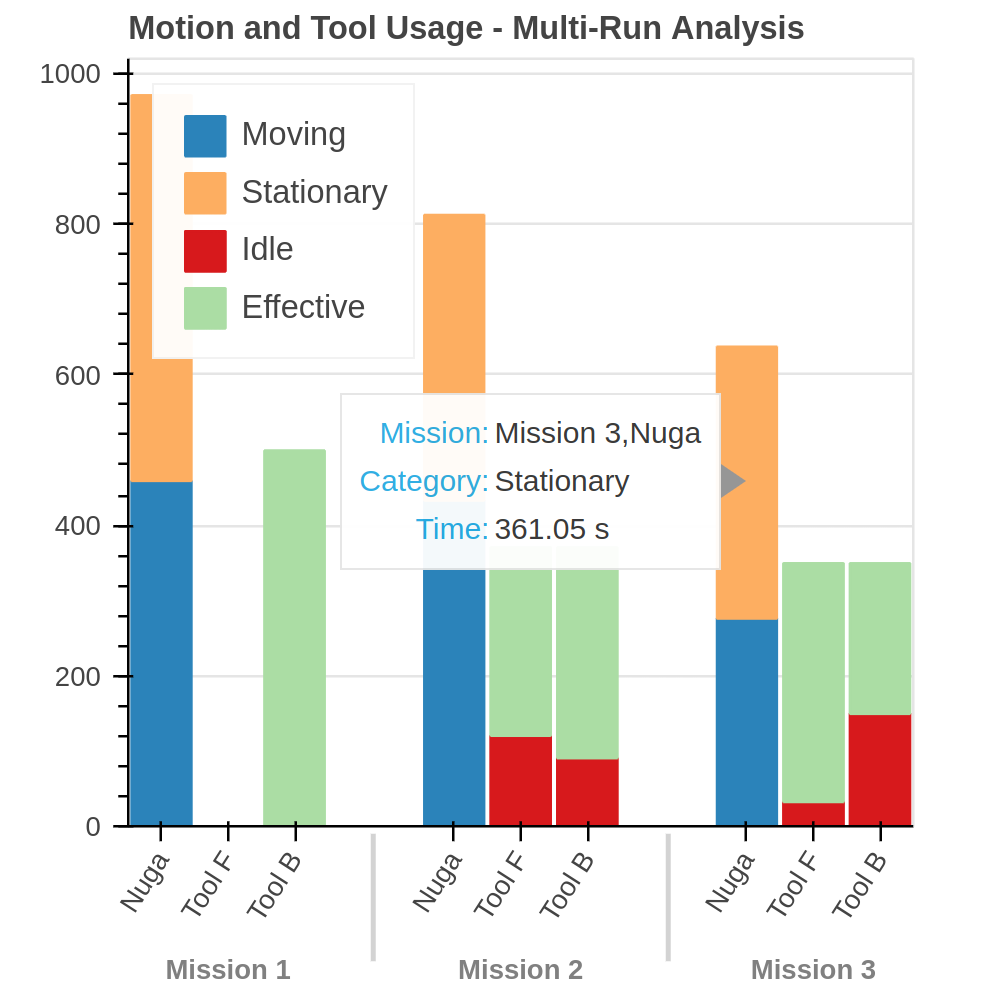
\includegraphics[width=.45\linewidth]{gfx/ch03/mission_metrics.png}} \quad
    \subfloat[Task Visualization]
    {\label{fig:heuristics-1-task-visualization}%
        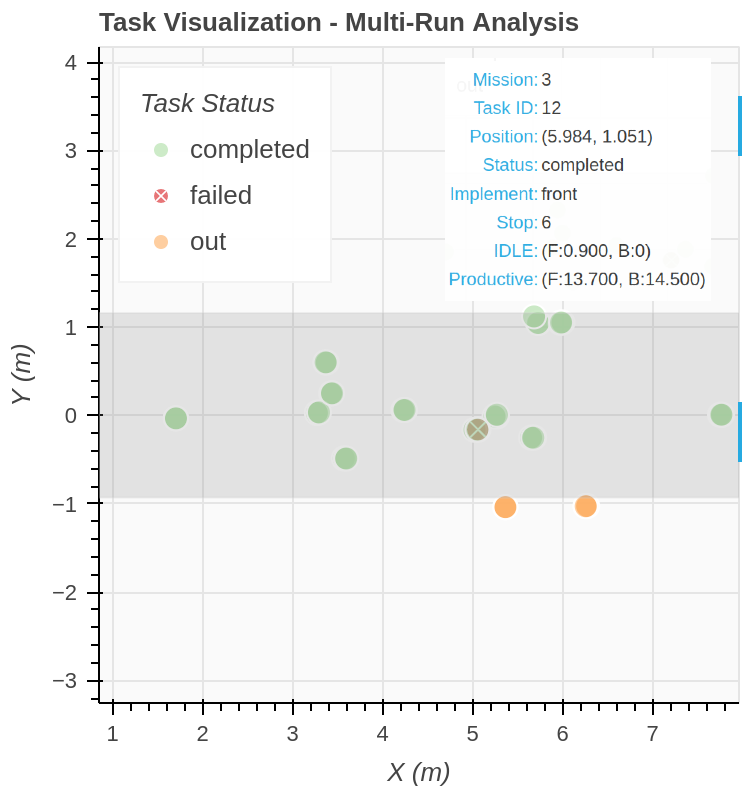
\includegraphics[width=.45\linewidth]{gfx/ch03/task_metrics.png}} \\
    \caption{Heuristics 1 tool vs 2 tools}\label{fig:heuristic-1tools-vs-2tools}
\end{figure}

The mission improvement by just adding an additional tool is about $50\%$ in terms of mission time. 

The second comparison was made between all other methods using both tools in the same environment and the results are shown in \autoref{}.